\documentclass[10pt]{article}
\usepackage[landscape,margin=0.65in]{geometry}
\usepackage[T1]{fontenc}
\usepackage[utf8]{inputenc}
\usepackage{tikz}
\usetikzlibrary{arrows.meta,positioning,fit}
\usepackage{tabularx}
\usepackage{array}
\usepackage[table]{xcolor}
\usepackage{hyperref}

\pagestyle{plain}
\setlength{\parindent}{0pt}
\setlength{\parskip}{4pt}
\renewcommand{\arraystretch}{1.12}
\hypersetup{colorlinks=true,linkcolor=blue,urlcolor=blue}

\definecolor{mizoreblue}{HTML}{245B9E}
\definecolor{lightblue}{HTML}{EAF2FB}
\definecolor{lightgray}{HTML}{F1F3F5}
\definecolor{riskcolor}{HTML}{FFF4DC}

\tikzset{
  component/.style={draw=mizoreblue, rounded corners, fill=lightblue,
    line width=0.8pt, minimum width=3.7cm, minimum height=1.15cm,
    align=center, font=\small},
  store/.style={draw=gray!75, rounded corners, fill=lightgray,
    line width=0.8pt, minimum width=3.7cm, minimum height=1.15cm,
    align=center, font=\small},
  actor/.style={draw=gray!75, rounded corners, fill=white,
    line width=0.8pt, minimum width=3.3cm, minimum height=1.15cm,
    align=center, font=\small},
  edge/.style={-{Stealth[length=2mm]}, thick},
  boundary/.style={draw=gray!70, dashed, rounded corners, inner sep=12pt},
  layer/.style={draw=mizoreblue, rounded corners, fill=lightblue,
    minimum width=3.2cm, minimum height=0.9cm, align=center, font=\small},
  entity/.style={draw=mizoreblue, line width=0.8pt, fill=white, inner sep=0pt,
    font=\small},
  rel/.style={thick, draw=mizoreblue},
  card/.style={font=\scriptsize, fill=white, inner sep=1.5pt}
}

% Entity box: #1 = table name, #2 = tabular rows (key & column & type \\)
\newcommand{\erentity}[2]{%
  \begin{tabular}{@{\hspace{4pt}}l@{\hspace{6pt}}l@{\hspace{10pt}}l@{\hspace{4pt}}}
    \multicolumn{3}{@{}c@{}}{\cellcolor{lightblue}\rule{0pt}{12pt}\textbf{\texttt{#1}}} \\[2pt]
    \hline
    \rule{0pt}{11pt}#2
  \end{tabular}}
\newcommand{\pk}{\textbf{\scriptsize PK}}
\newcommand{\fk}{\textit{\scriptsize FK}}

\begin{document}

\begin{center}
  {\LARGE\bfseries Mizore}\\[2pt]
  {\Large Software Architecture Document}\\[4pt]
  {\small Architecture description of the current repository implementation}
\end{center}

\begin{center}
\begin{tabularx}{0.82\linewidth}{>{\bfseries}p{3.2cm}X
                                 >{\bfseries}p{2.6cm}X}
Document status & Draft & Version & 1.1 \\
System & Mizore & Source basis & Commit \texttt{7009fb2} (multi-root shared folders) \\
\end{tabularx}
\end{center}

\tableofcontents
\newpage

\section{Introduction}

\subsection{Purpose}
This document describes Mizore's architecture: its system boundary, runtime components,
responsibility allocation, data stores, interfaces, deployment shape, and notable constraints.
It is a description of the current implementation, not a feature specification or a proposal
for an unimplemented target architecture.

\subsection{Scope}
Mizore is a self-hosted, browser-based file browser. Users sign in, register saved
\emph{paths} (folders inside one of the server's shared roots), and browse or view the files
in them, including PDFs. The architecture in scope includes the Next.js frontend, the Fastify
API, the PostgreSQL database, and the host directories bind-mounted into the backend as
shared roots.

\subsection{Audience}
This document is intended for developers, maintainers, and operators who need to locate
responsibilities, understand service interactions, or assess the impact of a change.

\subsection{Conventions}
The architecture views are implementation-oriented. Solid arrows indicate runtime requests or
data access. A dashed boundary indicates services grouped by Docker Compose. Statements marked
as current behavior describe the checked-in code and may include known gaps.

\section{Architecture Drivers}

\subsection{Stakeholders and concerns}
\begin{tabularx}{\linewidth}{>{\raggedright\arraybackslash\bfseries}p{4cm}X}
Stakeholder & Primary architecture concern \\
\hline
Browser user & Sign in, access saved paths, and browse or preview files through the web UI. \\
Owner or admin & Manage users and perform administrative operations. \\
Developer or maintainer & Change UI, API, persistence, or file handling without crossing layer boundaries accidentally. \\
Operator & Configure ports, database connection, JWT secrets, the API proxy target, and which host folders are exposed as shared roots. \\
\end{tabularx}

\subsection{Key use cases}
\begin{enumerate}
  \item Authenticate with username and password and restore a client session.
  \item List the mounted shared roots and create, update, and delete a user's saved paths.
  \item List a directory and retrieve a file (including PDF preview) from any configured shared root.
  \item Perform user-administration operations subject to the configured role checks.
\end{enumerate}

\subsection{Constraints and assumptions}
\begin{itemize}
  \item The frontend and backend are separate services. The browser only talks to Next.js;
  Next.js rewrites \texttt{/api/*} to the backend at \texttt{API\_PROXY\_TARGET}
  (default \texttt{http://localhost:4000}, \texttt{http://backend:4000} in Compose).
  \item PostgreSQL stores application records. File contents remain on the host filesystem.
  \item One or more host directories act as shared roots, configured by
  \texttt{SHARED\_FOLDERS} (comma-separated) or the legacy single \texttt{SHARED\_FOLDER};
  the backend falls back to \texttt{/files} when neither is set.
  \item In Docker, each root is bind-mounted with target equal to source so that paths stored in
  the database are the same as host paths.
  \item The checked-in deployment uses Docker Compose, PostgreSQL 16, and Node.js 20 images.
  \item No formal service-level objectives, capacity targets, or availability targets are stated
  in the repository documentation.
\end{itemize}

\section{System Context and Container View}

Mizore is used through a browser. The browser loads the UI from Next.js and sends relative
\texttt{/api/...} requests to the same origin; Next.js forwards them to Fastify. Fastify reads and
writes PostgreSQL records and accesses files beneath its configured shared roots. The database
and the shared roots are resources used by the application; neither is a separate user-facing
service.

\begin{center}
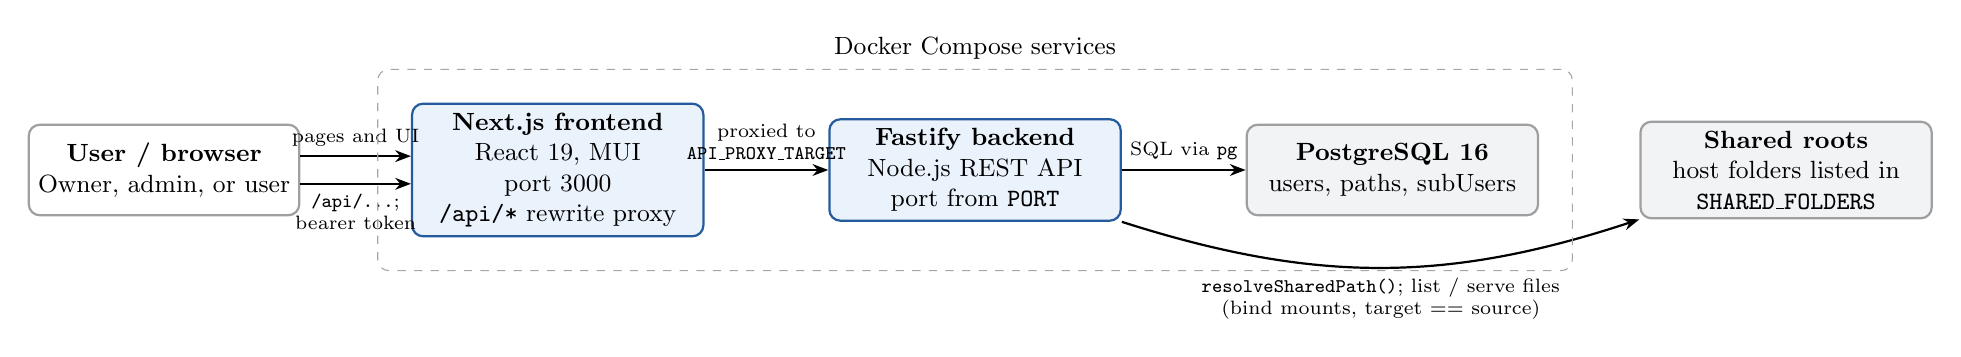
\begin{tikzpicture}[x=1cm,y=1cm]
  \node[actor] (browser) at (0,0) {\textbf{User / browser}\\Owner, admin, or user};
  \node[component] (web) at (5,0) {\textbf{Next.js frontend}\\React 19, MUI\\port 3000\\\texttt{/api/*} rewrite proxy};
  \node[component] (api) at (10.3,0) {\textbf{Fastify backend}\\Node.js REST API\\port from \texttt{PORT}};
  \node[store] (db) at (15.6,0) {\textbf{PostgreSQL 16}\\users, paths, subUsers};
  \node[store] (files) at (20.6,0) {\textbf{Shared roots}\\host folders listed in\\\texttt{SHARED\_FOLDERS}};

  \draw[edge] ([yshift=5pt]browser.east) -- node[above,font=\scriptsize,align=center]
    {pages and UI} ([yshift=5pt]web.west);
  \draw[edge] ([yshift=-5pt]browser.east) -- node[below,font=\scriptsize,align=center]
    {\texttt{/api/...};\\bearer token} ([yshift=-5pt]web.west);
  \draw[edge] (web.east) -- node[above,font=\scriptsize,align=center]
    {proxied to\\\texttt{API\_PROXY\_TARGET}} (api.west);
  \draw[edge] (api.east) -- node[above,font=\scriptsize,align=center]
    {SQL via \texttt{pg}} (db.west);
  \draw[edge] (api.south east) to[bend right=18]
    node[below,font=\scriptsize,align=center]
    {\texttt{resolveSharedPath()}; list / serve files\\(bind mounts, target == source)} (files.south west);

  \node[boundary,fit=(web)(api)(db),label={[font=\small]above:Docker Compose services}]
    (compose) {};
\end{tikzpicture}
\end{center}

\section{Architecture Views}

\subsection{Logical and component view}
The backend follows a route--controller--service--model organization. Route modules map HTTP
paths and attach pre-handlers; controllers validate input and map errors to HTTP status codes;
services implement operations; models issue parameterized SQL queries. Authentication is
implemented in \texttt{auth.controller.js} (\texttt{authenticate}) and
\texttt{user.controller.js} (\texttt{requireAdmin}). \texttt{config/storage.js} is the single
source of truth for which host directories are reachable: every filesystem access derived from
user input goes through \texttt{resolveSharedPath()}. The frontend separates pages, reusable
components, and shared client state.

\begin{center}
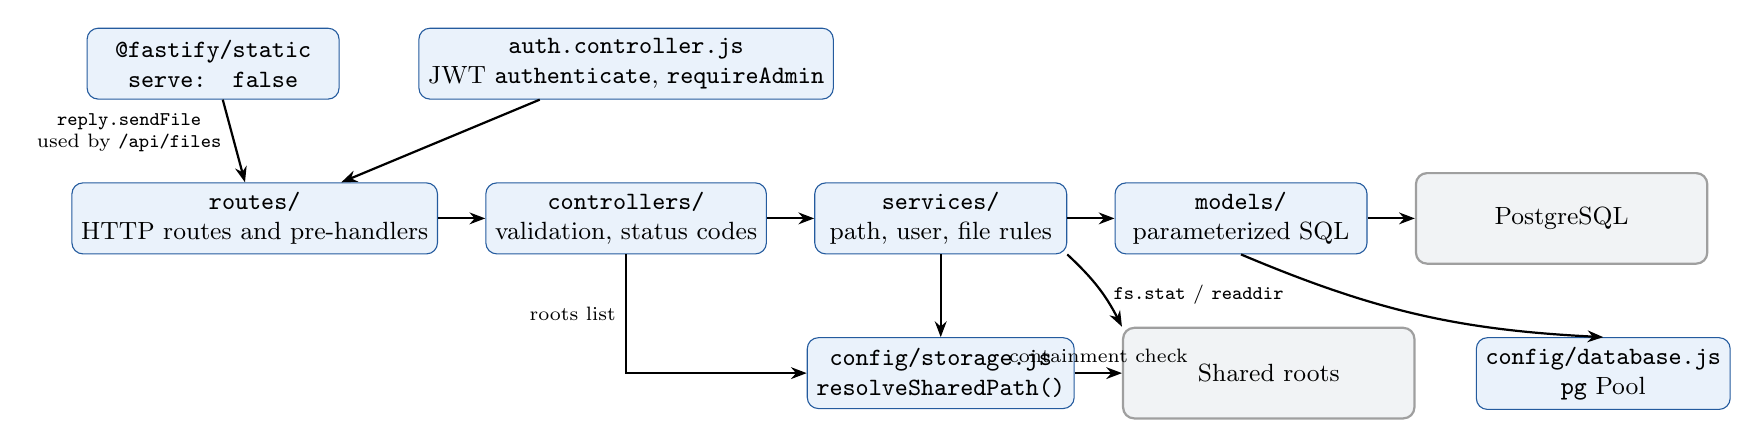
\begin{tikzpicture}[node distance=0.55cm and 0.6cm]
  \node[layer] (routes) {\texttt{routes/}\\HTTP routes and pre-handlers};
  \node[layer,right=of routes] (controllers) {\texttt{controllers/}\\validation, status codes};
  \node[layer,right=of controllers] (services) {\texttt{services/}\\path, user, file rules};
  \node[layer,right=of services] (models) {\texttt{models/}\\parameterized SQL};
  \node[store,right=of models] (postgres) {PostgreSQL};

  \draw[edge] (routes) -- (controllers);
  \draw[edge] (controllers) -- (services);
  \draw[edge] (services) -- (models);
  \draw[edge] (models) -- (postgres);

  \node[layer,below=1.05cm of services] (storage) {\texttt{config/storage.js}\\\texttt{resolveSharedPath()}};
  \node[store,right=of storage] (filesystem) {Shared roots};
  \node[layer,below=1.05cm of models,xshift=4.6cm] (dbcfg) {\texttt{config/database.js}\\\texttt{pg} Pool};
  \draw[edge] (services) -- (storage);
  \draw[edge] (controllers.south) |- node[pos=0.25,left,font=\scriptsize]{roots list} (storage.west);
  \draw[edge] (storage) -- node[above,font=\scriptsize]{containment check} (filesystem);
  \draw[edge] (services.south east) to[bend left=10] node[right,font=\scriptsize,pos=0.6]{\texttt{fs.stat} / \texttt{readdir}} (filesystem.north west);
  \draw[edge] (models.south) to[bend right=10] (dbcfg.north);

  \node[layer,above=1.05cm of controllers] (auth) {\texttt{auth.controller.js}\\JWT \texttt{authenticate}, \texttt{requireAdmin}};
  \draw[edge] (auth) -- (routes);
  \node[layer,left=1.0cm of auth] (static) {\texttt{@fastify/static}\\\texttt{serve: false}};
  \draw[edge] (static) -- node[left,font=\scriptsize,align=center,pos=0.4]{\texttt{reply.sendFile}\\used by \texttt{/api/files}} (routes);
\end{tikzpicture}
\end{center}

\small
\begin{tabularx}{\linewidth}{>{\raggedright\arraybackslash}p{4.3cm}
                              >{\raggedright\arraybackslash}X
                              >{\raggedright\arraybackslash}X}
\textbf{Component} & \textbf{Location and responsibility} & \textbf{Boundary} \\
\hline
Frontend pages & \texttt{nextjs/src/app/}; login, user creation, admin (guarded by \texttt{adminGuard.tsx}), catch-all file browser \texttt{admin/[...path]}, PDF viewer, and settings. &
UI and page composition; API calls are relative \texttt{/api/...} URLs. \\
Frontend shared state & \texttt{nextjs/src/context/AppContext.jsx}; tokens, user, saved paths, shared roots, current path, and the authenticated \texttt{request()} helper. &
App context owns client-side authentication and path state. \\
Sidebar & \texttt{nextjs/src/components/sidebar/}; path list grouped by root (\texttt{groupPathsByRoot}), add/edit dialog with source picker, delete dialog. &
Mirrors backend root resolution; must change together with \texttt{storage.js}. \\
API proxy & \texttt{nextjs/next.config.ts} rewrites \texttt{/api/:path*} to \texttt{API\_PROXY\_TARGET}. &
Single browser-visible origin; backend need not be reachable from the browser. \\
HTTP API & \texttt{node\_fastify/src/routes/} and \texttt{controllers/}; auth, user, path, source, and file endpoints. &
Routes define pre-handlers; controllers handle HTTP-level concerns and \texttt{\{ error \}} responses. \\
Application logic & \texttt{node\_fastify/src/services/}; path, user, and file operations. &
Coordinates data access and filesystem operations. \\
Shared-root configuration & \texttt{node\_fastify/src/config/storage.js}. &
Parses roots, resolves absolute / slash-less / legacy-relative paths, most specific root wins, rejects anything outside. \\
Persistence & \texttt{node\_fastify/src/models/} and \texttt{config/database.js}. &
Parameterized SQL over a shared \texttt{pg} connection pool. \\
Database schema & \texttt{postgres/init.sql} and \texttt{postgres/migrations/}. &
Initialization applies to an empty volume; existing databases require migrations. \\
\end{tabularx}
\normalsize

\subsection{Runtime view}
\textbf{Authentication flow.} The browser posts credentials to \texttt{/api/login}. The API
loads the user record (case-insensitive username), compares the bcrypt hash, and returns a user
object and access/refresh JWTs. The client stores the tokens and the user in local storage and
sends the access token as a bearer token through \texttt{request()}. On page load the client
restores the stored session and calls \texttt{/api/me}; a 401 or 403 clears the session.

\textbf{Saved-path flow.} After the session is restored, the client calls
\texttt{GET /api/paths/:userId}, which returns the user's paths and the list of shared
\texttt{roots}; the sidebar groups paths under their root. The add/edit dialog loads
\texttt{GET /api/sources}, lets the user pick a source root and a folder inside it, and sends
the joined absolute path. Path creation runs \texttt{resolveSharedPath()}, checks that the target
exists and is a directory, then inserts the record. Update and delete are \texttt{PATCH} /
\texttt{DELETE /api/paths/:id}.

\textbf{File-browsing flow.} The client lists a folder through \texttt{/api/list/:file} and
fetches file content (for example a PDF cover preview or the full PDF viewer) through
\texttt{/api/files/:filename}. Both resolve the encoded path with \texttt{resolveSharedPath()}:
an outside path returns 400, a missing one 404. Listing uses \texttt{fs.readdir}; file content is
streamed by \texttt{reply.sendFile(relativePath, root)}. Whether a user may open sub-folders of a
saved path (\texttt{allowed\_subpath}) is enforced only in the UI.

\subsection{Deployment view}
The Compose deployment contains frontend, backend, and PostgreSQL services. PostgreSQL uses
the \texttt{postgres\_data} named volume and initializes from \texttt{postgres/init.sql};
the backend waits for the database health check. The backend image starts
\texttt{node server.js} and receives \texttt{SHARED\_FOLDER} / \texttt{SHARED\_FOLDERS}; each host
folder to expose is bind-mounted into the backend with target equal to source
(\texttt{create\_host\_path: false}). The frontend uses a multi-stage Next.js build that takes
\texttt{API\_PROXY\_TARGET} as a build argument and environment variable, and serves on port 3000.
Only the frontend needs to be reachable by browsers.

\subsection{Data view}
The PostgreSQL schema defined in \texttt{postgres/init.sql} (with
\texttt{migrations/001\_add\_allowed\_subpath.sql}) contains three tables. Both
\texttt{paths} and \texttt{subUsers} reference \texttt{users.id}; there are no relationships
between \texttt{paths} and \texttt{subUsers}. File contents are not part of the schema.
\texttt{paths.path} holds an absolute host path inside a shared root (older rows may hold a path
relative to the first root).

\begin{center}
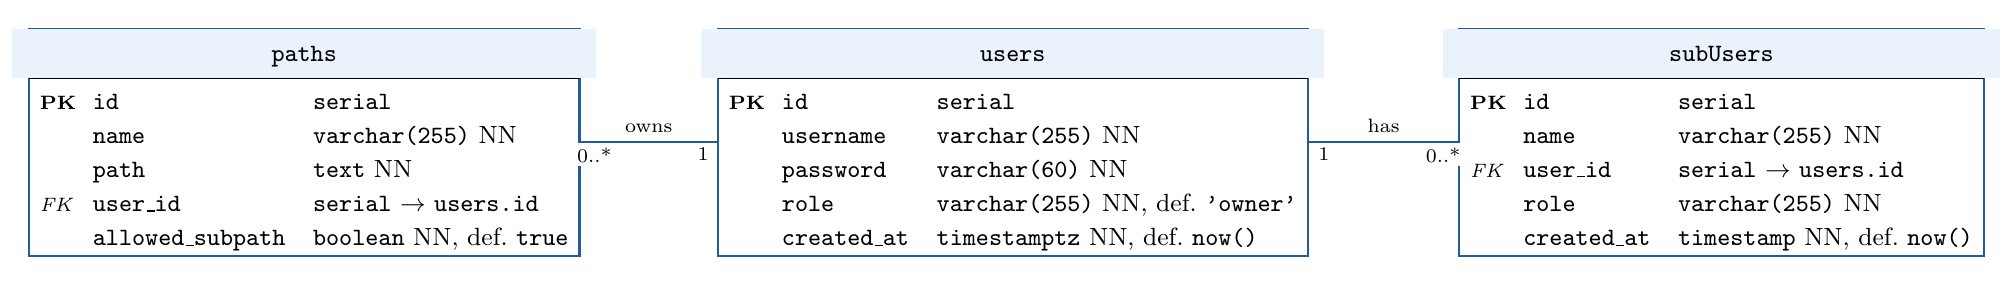
\begin{tikzpicture}
  \node[entity] (users) at (0,0) {\erentity{users}{%
    \pk & \texttt{id} & \texttt{serial} \\
        & \texttt{username} & \texttt{varchar(255)} NN \\
        & \texttt{password} & \texttt{varchar(60)} NN \\
        & \texttt{role} & \texttt{varchar(255)} NN, def.\ \texttt{'owner'} \\
        & \texttt{created\_at} & \texttt{timestamptz} NN, def.\ \texttt{now()} \\}};

  \node[entity] (paths) at (-9,0) {\erentity{paths}{%
    \pk & \texttt{id} & \texttt{serial} \\
        & \texttt{name} & \texttt{varchar(255)} NN \\
        & \texttt{path} & \texttt{text} NN \\
    \fk & \texttt{user\_id} & \texttt{serial} $\rightarrow$ \texttt{users.id} \\
        & \texttt{allowed\_subpath} & \texttt{boolean} NN, def.\ \texttt{true} \\}};

  \node[entity] (subusers) at (9,0) {\erentity{subUsers}{%
    \pk & \texttt{id} & \texttt{serial} \\
        & \texttt{name} & \texttt{varchar(255)} NN \\
    \fk & \texttt{user\_id} & \texttt{serial} $\rightarrow$ \texttt{users.id} \\
        & \texttt{role} & \texttt{varchar(255)} NN \\
        & \texttt{created\_at} & \texttt{timestamp} NN, def.\ \texttt{now()} \\}};

  \draw[rel] (users.west) -- node[above,font=\scriptsize]{owns}
    node[pos=0.1,below,card]{1} node[pos=0.9,below,card]{0..*} (paths.east);
  \draw[rel] (users.east) -- node[above,font=\scriptsize]{has}
    node[pos=0.1,below,card]{1} node[pos=0.9,below,card]{0..*} (subusers.west);
\end{tikzpicture}

{\scriptsize PK = primary key; FK = foreign key; NN = \texttt{NOT NULL}; def.\ = default.
Cardinality: one user to zero or more rows.}
\end{center}

\begin{tabularx}{\linewidth}{>{\raggedright\arraybackslash}p{3.8cm}
                              >{\raggedright\arraybackslash}X
                              >{\raggedright\arraybackslash}X}
\textbf{Store / entity} & \textbf{Data} & \textbf{Relationship / use} \\
\hline
\texttt{users} & ID, username, password hash, role, creation time. &
Account records; roles include values used by route checks, such as \texttt{admin} and \texttt{owner}. The app is intended to have at most one owner. \\
\texttt{subUsers} & ID, name, role, parent user ID, creation time. &
Subordinate records associated with a user; usernames are checked for uniqueness across both tables. \\
\texttt{paths} & ID, name, path, user ID, \texttt{allowed\_subpath}. &
Saved directory metadata associated with a user. \\
Shared roots & Directory entries and file bytes. &
Read by the backend; the set of roots comes from environment configuration, not the database. \\
\end{tabularx}

\subsection{Interface view}
\small
\begin{tabularx}{\linewidth}{>{\raggedright\arraybackslash}p{3.6cm}
                              >{\raggedright\arraybackslash}X
                              >{\raggedright\arraybackslash}p{6.2cm}}
\textbf{Interface} & \textbf{Endpoints / examples} & \textbf{Guard / notes} \\
\hline
Browser--frontend & HTTP pages and client-side UI. & Same origin also serves \texttt{/api/*}. \\
Frontend--API (proxy) & Next.js rewrite \texttt{/api/:path*} $\rightarrow$ \texttt{API\_PROXY\_TARGET}. & Request and \texttt{Authorization} header passed through. \\
Auth & \texttt{POST /api/login}, \texttt{GET /api/me}. & Login public; \texttt{/me} requires \texttt{authenticate}. \\
Paths & \texttt{GET /api/paths/:userId} (returns \texttt{paths} and \texttt{roots}), \texttt{POST /api/paths}, \texttt{PATCH /api/paths/:id}, \texttt{DELETE /api/paths/:id}. & \texttt{authenticate}. \\
Sources & \texttt{GET /api/sources} (returns \texttt{sources}: configured roots). & \texttt{authenticate}. \\
Files & \texttt{GET /api/list/:file}, \texttt{GET /api/files/:filename}. & No pre-handler; path checked by \texttt{resolveSharedPath()}. \\
Users & \texttt{GET /api/users}, \texttt{GET /api/users/:username}, \texttt{POST /api/users/createdSubUser}, \texttt{PATCH|PUT|DELETE /api/users/:id}. & \texttt{requireAdmin} (\texttt{admin} or \texttt{owner}). \\
User sign-up & \texttt{POST /api/users/createdUser}. & No pre-handler. \\
API--database & PostgreSQL protocol through the \texttt{pg} pool. & Parameterized SQL only. \\
API--filesystem & \texttt{fs.stat}, \texttt{fs.readdir}, \texttt{reply.sendFile} under a shared root. & Every user path resolved by \texttt{resolveSharedPath()}. \\
\end{tabularx}
\normalsize

\section{Cross-Cutting Concerns}

\subsection{Authentication and authorization}
Access tokens are signed as JWTs with a one-hour expiry; refresh tokens have a seven-day
expiry. Path, source, and current-user routes install \texttt{authenticate}. User-administration
routes require \texttt{admin} or \texttt{owner} through \texttt{requireAdmin}. The admin UI is
gated client-side to the same roles. Token verification is performed by the backend.

\subsection{File-path boundary}
\texttt{config/storage.js} normalizes the configured roots and resolves any user-supplied path to
an absolute path inside one of them, preferring the most specific root when roots are nested.
It accepts absolute paths, absolute paths without the leading slash (the frontend strips it when
building URLs), and legacy paths relative to the first root, and throws
\texttt{'Path is outside the shared folder'} otherwise. Path creation, directory listing, and file
serving all use it; \texttt{@fastify/static} is registered with \texttt{serve: false} so no file is
reachable except through \texttt{/api/files}. The frontend duplicates the root-matching logic in
\texttt{groupPathsByRoot} (\texttt{sidebar/utils.ts}) and \texttt{splitSourcePath}
(\texttt{sidebar/addpath.tsx}).

\subsection{Persistence and migration}
PostgreSQL schema initialization is performed by \texttt{postgres/init.sql} when the data
volume is first created. The \texttt{allowed\_subpath} column is also represented by a migration
for databases that already exist. New schema changes are added as numbered, idempotent files in
\texttt{postgres/migrations/} and mirrored in \texttt{init.sql}.

\subsection{Testing}
Backend integration tests (\texttt{node:test} with \texttt{app.inject()}) create two temporary
shared roots and set \texttt{SHARED\_FOLDERS} before importing the app. They cover listing and
downloading from either root, long encoded nested paths, rejection of paths outside every root,
and the authenticated \texttt{/api/sources} endpoint. Tests that reach the database require a
running PostgreSQL.

\section{Architecture Decisions and Rationale}
\begin{tabularx}{\linewidth}{>{\raggedright\arraybackslash\bfseries}p{4.2cm}X}
Decision reflected in code & Rationale or observed consequence \\
\hline
Separate frontend and API services & UI and API can be built and started independently. \\
Same-origin API through a Next.js rewrite & The browser calls relative \texttt{/api/...} URLs, so no public backend URL or CORS setup is needed for the browser; the proxy target is fixed at build/start time. \\
PostgreSQL for application records & Relational user and saved-path data is kept separately from the contents being browsed. \\
Multiple shared roots with one resolver & Several host folders can be exposed; a single \texttt{resolveSharedPath()} keeps the traversal check in one place. \\
Bind mounts with target == source & Paths saved in the database are identical inside and outside the container. \\
Layered Fastify backend & Routes, controllers, services, and models have distinct HTTP, application, and persistence responsibilities. \\
Bearer JWT session & The client can authenticate API requests without a server-side session store; tokens are currently stored in browser local storage. \\
\end{tabularx}

\section{Quality Attribute Assessment}
The repository does not define measurable quality-attribute targets. The following table records
the design mechanisms and the current evidence or limitation rather than claiming that a target
has been met.

\begin{tabularx}{\linewidth}{>{\bfseries}p{3.5cm}X X}
Attribute & Current mechanism & Assessment / evidence \\
\hline
Security & bcrypt password hashing, bearer JWT authentication, role checks, shared-root containment in \texttt{resolveSharedPath()}, static serving disabled. &
Traversal outside the roots is rejected and covered by tests. File-list and file-download routes are still unauthenticated, and path routes do not check ownership. \\
Data durability & PostgreSQL named volume. &
Database data persists across container recreation; initialization scripts do not automatically migrate existing volumes. \\
Modifiability & Layered backend, separate frontend/backend projects, single root resolver. &
Root resolution is duplicated in the frontend and must be kept in sync. \\
Operability & Fastify logging and PostgreSQL health check. &
No centralized monitoring, backup policy, or formal availability target is specified in the repository. \\
\end{tabularx}

\section{Risks and Open Issues}
\begin{itemize}
  \setlength\itemsep{2pt}
  \item \textbf{Shared-root configuration:} Compose bind-mounts specific host folders, but
  \texttt{SHARED\_FOLDERS} defaults to empty and \texttt{SHARED\_FOLDER} to \texttt{/files}. Unless
  \texttt{.env} lists every mount target in \texttt{SHARED\_FOLDERS}, the backend's roots do not
  match the mounted folders.
  \item \textbf{Proxy target and port:} Compose defaults \texttt{API\_PROXY\_TARGET} to
  \texttt{http://backend:4000} while the backend listens on \texttt{BACKEND\_PORT}; these must
  agree.
  \item \textbf{File-route authorization:} \texttt{/api/list/:file} and
  \texttt{/api/files/:filename} do not install authentication pre-handlers. Anyone who can reach
  the frontend can list and download any file inside any shared root, regardless of saved paths
  or \texttt{allowed\_subpath} (which is enforced only in the UI).
  \item \textbf{Path ownership:} \texttt{GET /api/paths/:userId}, \texttt{PATCH} and
  \texttt{DELETE /api/paths/:id} require a valid token but do not check that the path or user ID
  belongs to the caller.
  \item \textbf{Path update validation:} path creation runs \texttt{resolveSharedPath()} and
  checks directory existence; the update operation writes path metadata without those checks.
  \item \textbf{Open user creation:} \texttt{POST /api/users/createdUser} has no pre-handler and
  accepts a \texttt{role}, so the ``at most one owner'' rule is not enforced by the backend.
  \item \textbf{User update without password:} \texttt{User.updateById} always writes
  \texttt{password}; when the request omits it (as the settings edit dialog does), \texttt{NULL}
  is written to a \texttt{NOT NULL} column and the update fails.
  \item \textbf{Refresh behavior:} the client stores a refresh token, but the current route set
  does not expose a refresh endpoint; an expired access token ends the session.
  \item \textbf{Duplicate session loading:} the sidebar hook \texttt{useLoadUserAndPaths} and
  \texttt{AppContext} each call \texttt{/api/me} and \texttt{/api/paths/:userId}.
  \item \textbf{\texttt{subUsers} schema mismatch:} \texttt{subUser.model.js} inserts a
  \texttt{password} column that \texttt{postgres/init.sql} does not define, so sub-user creation
  fails against the initialized schema. In addition, the \texttt{user\_id} foreign keys in
  \texttt{paths} and \texttt{subUsers} are declared as \texttt{serial}, which attaches an
  unintended sequence default; \texttt{integer} is the usual type for a foreign key.
\end{itemize}

\section{Glossary}
\begin{tabularx}{\linewidth}{>{\bfseries}p{4cm}X}
API & Application Programming Interface; in this system, the Fastify HTTP endpoints. \\
JWT & JSON Web Token used by the API to authenticate bearer-token requests. \\
Shared root / source & A host directory the backend may access, configured through \texttt{SHARED\_FOLDERS} (or \texttt{SHARED\_FOLDER}); returned to the UI as \texttt{roots} / \texttt{sources}. \\
Saved path & A PostgreSQL record identifying a directory inside a shared root that a user sees in the sidebar. \\
\end{tabularx}

\section{References}
\begin{itemize}
  \item \texttt{README.md} and \texttt{AGENTS.md} --- project overview, commands, and conventions.
  \item \texttt{DOCKER\_DEPLOYMENT.md} --- deployment configuration and migration notes.
  \item \texttt{docker-compose.yml} and \texttt{.env.example} --- service topology, mounts, and variables.
  \item \texttt{node\_fastify/src/} --- API routes, controllers, services, models, configuration, and tests.
  \item \texttt{nextjs/src/} and \texttt{nextjs/next.config.ts} --- frontend pages, components, client state, and API proxy.
  \item \texttt{postgres/init.sql} and \texttt{postgres/migrations/} --- database schema and migration.
\end{itemize}

\end{document}
